\section{Feature Engineering}
\subsection{Data Peparation and Exploration (EDA)}
Though exploratory data analysis (EDA) we can often:
\begin{itemize}
    \item discover important anomalies
    \item identify limitations in the collection process
    \item and better inform subsequent goal oriented analysis
\end{itemize}
Perpare, analyze and visualize data by unsing:
\begin{itemize}
    \item Histogramm, QQ-Plot
    \item Scatter-Matrix
    \item countplots, contingency tables
    \item Heatmaps
\end{itemize}

\subsection{Feature Preparation/generation}
\begin{itemize}
    \item Data \textbf{Cleaning}: Homogenize missing values and different types of the same feature, fix input errors, types, etc.
    \item \textbf{Aggregation|Pivoting}: Necessary when the entity to model is an aggregation from the provided data.
    \item \textbf{Imputation }of missing values. Strategies: mean, median, mode, using a model
    \item \textbf{Binarization}: Transform discrete or continuous numeric features into binary features
    \item \textbf{Binning} (fixed width, adaptive quantile binning): Split numerical values into bins and encode with a bin ID 
    \item \textbf{Transformation}(eg. Log-Transform, BoxCox): Compress the range of large numbers or expand the range of small numbers.
    \item \textbf{Scaling} and \textbf{normalizing} (min/max,z-score): Scale numerical variables into a certain range.
    \item \textbf{Generate Interaction features }
\end{itemize}
\subsection{Feature selection}
There are general two reasons why feature selection is used:
\begin{enumerate}
    \item Reducing the number of features, to reduce overfitting and improve the generalization of models
    \item To gain a better understanding of the features and their relationship to the response variables
\end{enumerate}
These two goals are often ar odds with each other.
\subsubsection{Univariate Feature Selection}
\begin{itemize}
    \item Based on univariate statistical tests.Examined for each feature individually
    \item Good for gaining a better understanding
    \item For regression: f\_regression, mutual\_info\_regression
    \item For classification: chi2, f\_classif, mutual\_info\_classif
\end{itemize}
Pearson Correlation Coefficient:
\[
\rho_{X_i,y} = \frac{\text{cov}[X_i,Y]}{\sigma_{X_i}\cdot \sigma_Y} = \frac{\mathbb{E}[X_i-\overline{X}_i]\cdot \mathbb{E}[Y-\overline{Y}]}{\sigma_{X_i}\cdot \sigma_Y}
\]
F-Regression test:
\[
\frac{\text{TSS}-\text{RSS}/p}{\text{RSS}/(n-p-1)} \sim F_{p,n-p-1}
\]
Mutual Information coefficant:
\[
I(X,Y) = \sum_{y \in Y} \sum_{x \in X} p(x,y)\cdot \log\left(\frac{p(x,y)}{p(x)\cdot p(y)}\right)
\]
\subsubsection{Feature selection using linear models \& regularization}
\begin{itemize}
    \item Lasso feature selection
    \item Ridge feature selection
    \item Linear Models: Subset selection
    \item Tree-based methods
\end{itemize}
\subsubsection*{Ridge feature selection}
Forces the coefficient values to be spread out more equally.
More usefull for feature interpertation then Lasso feature selection.

\subsubsection*{Linear Models}
Forward stepwise selection:
Let \(\mathcal{M}_0\) denote the null model with no predictors.
\begin{itemize}
    \item For \(k = 0,\dots,p-1\):
    \begin{enumerate}
        \item Consider all \((p-k)\) models that augment the perdictors in \(\mathcal{M}_k\) with one additional predictor.
        \item Choose the best among these \((p-k)\) models and call it \(\mathcal{M}_{k + 1}\). Here best is defined as having smallest \(RSS\) or highest \(R^2\).
    \end{enumerate}
    \item Select a single best model among \(\{\mathcal{M}_{0},\mathcal{M}_{1},\dots,\mathcal{M}_{p}\}\) using AIC or BIX or the adjusted \(R^2\)-score.
\end{itemize}
\subsubsection*{Metrics}
RSS = Residual Sum of Squares
\[
RSS = \sum_{i = 1}^{n}(y_i-\hat{y}_i)^2
\]
TSS = Total Sum of Squares
\[
    TSS = \sum_{i = 1}^{n}(y_i-\overline{y})^2
\]
\(R^2\)-score:(\% explained variance)
\[
R^2 = 1- \frac{RSS}{TSS}
\]
Adjusted \(R^2\)-score
\[
R^2_{adj} =  1- \frac{\frac{RSS}{n-p-1}}{\frac{TSS}{n-1}}
\]
AIC(Akaike) and BIC(Bayesian) Information Criteria, \(\mathcal{L}\): Likelihood
\[
AIC = -2\log(\mathcal{L}) + 2p \qquad BIC = -2\log(\mathcal{L}) + 2\log(n) \cdot p
\]

\subsection{Text data/Natural Lannguage Processing (NLP)}
Text analysis is a major application field for ML algorithms.
To feed text to a algorithms it first has to be transformd to a numerical vector by:
\begin{itemize}
    \item \textbf{Tokenizing:} strings and give an integer ID to each possible token
    \item \textbf{Counting:} the occurences of token in each documnet
    \item \textbf{Normalizing:} and weighting with diminishing importance tokens that occur in the majority of samples/documents
\end{itemize}
\subsubsection{Tokenization}
\begin{enumerate}
    \item All common seperators, operators, punctuations and non-printable characters are removed(using Regex).
    \item Then, stop-words filtering that aims to filter-out the most frequent words performed
    \item Finally, stemming and/or lemmatization is applied to obtain the stem of a word that is morphological root by removing the suffixes that present grammatical or lexical infromation about the word.
\end{enumerate}
\textbf{Porter Stemming:} Simple replacement rules to create word roots.

\textbf{Lemmatization:} seeks to find actual roots for words.(e.g., tome \(\rightarrow\) book)
\subsubsection{Word Embeddings}
Idea: Map one-hot encoding to dense vectors
\begin{itemize}
    \item Each word is represented using a low-dimensional, dense, real-valued vector that encodes the meaning of the word such that the words that are closer in the vector space are expected to be similar in meaning
    \item How to compute them? Can be pre-trained using a very general task on a very large corpus or learnt with the target task
\end{itemize}
\begin{figure}
    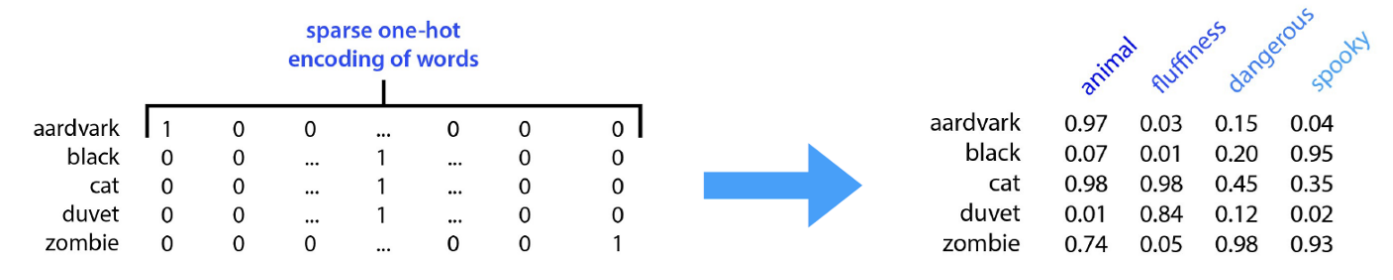
\includegraphics[width = \columnwidth]{figures/07/TextEmbeddings.png}
\end{figure}
This is called Word to vector(Word2Vec).
There are 2 variants:
\begin{itemize}
    \item continuous bad of words(CBOW)
    \item Skip-Gram
\end{itemize}
\subsection{Audio data}
In the time domain the resulting amplitudes, time delays (echos) are captured.
The fourier transform enables to decompose a signal into its individual frequencies an their amplitudes and phases.
\subsubsection{Linear predictive coding coefficients (LPC)}
LPC are parameters derived from audio signals that effectively model the spectral envelope of a sound wave.
They capture the articulatory constraints of the vocal tract.
\subsubsection{Spectogramm - Short Time Fourier Transform}
In many cases we have non periodic signals: frequency content varies over time. Compute FFT on overlapping windowed segments of the signal to obtain the spectogramm.
\begin{figure}[!h]
    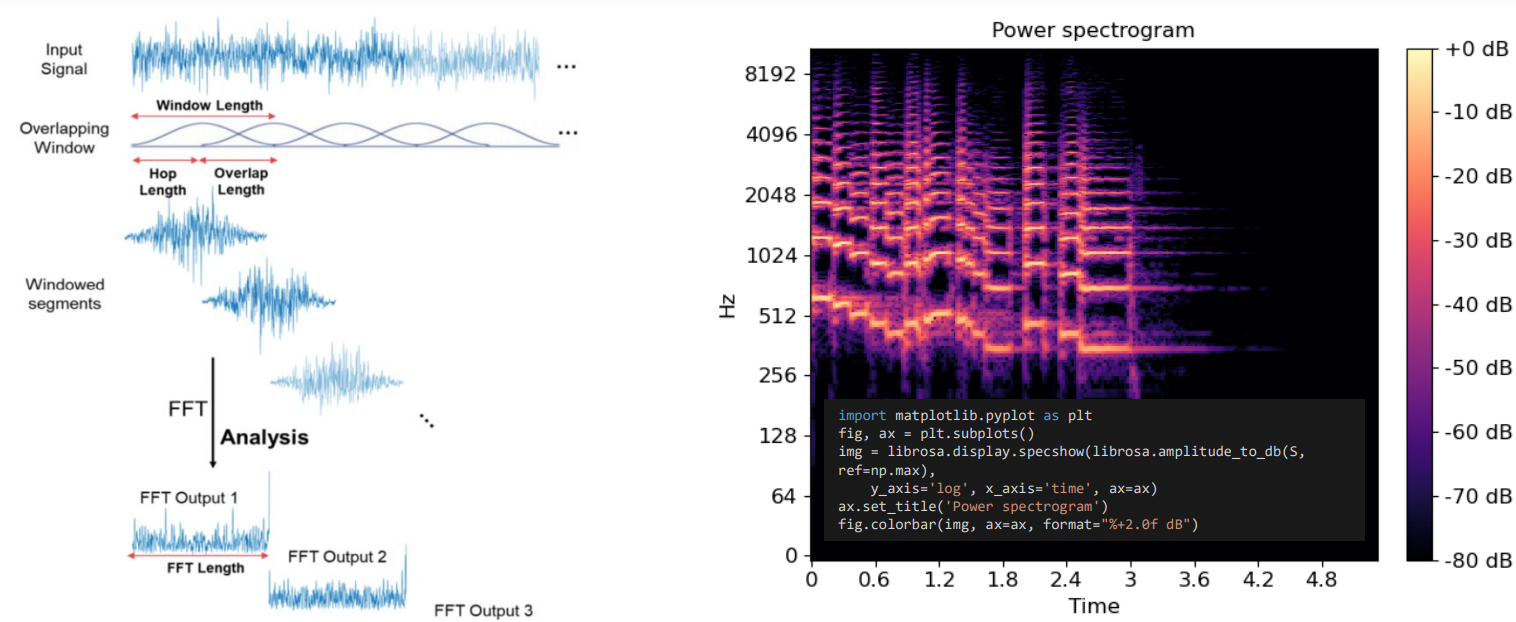
\includegraphics[width = \columnwidth]{figures/07/STFT.png}
\end{figure}
\subsubsection{Mel Frequency Cepstral Coefficients (MFCC)}
MFCC trys to mimic human hearing.
It condeses audio information into fewer coefficients, simplifying data without losing critical information.
They are noise robuster than raw spectral features.
\begin{figure}[!h]
    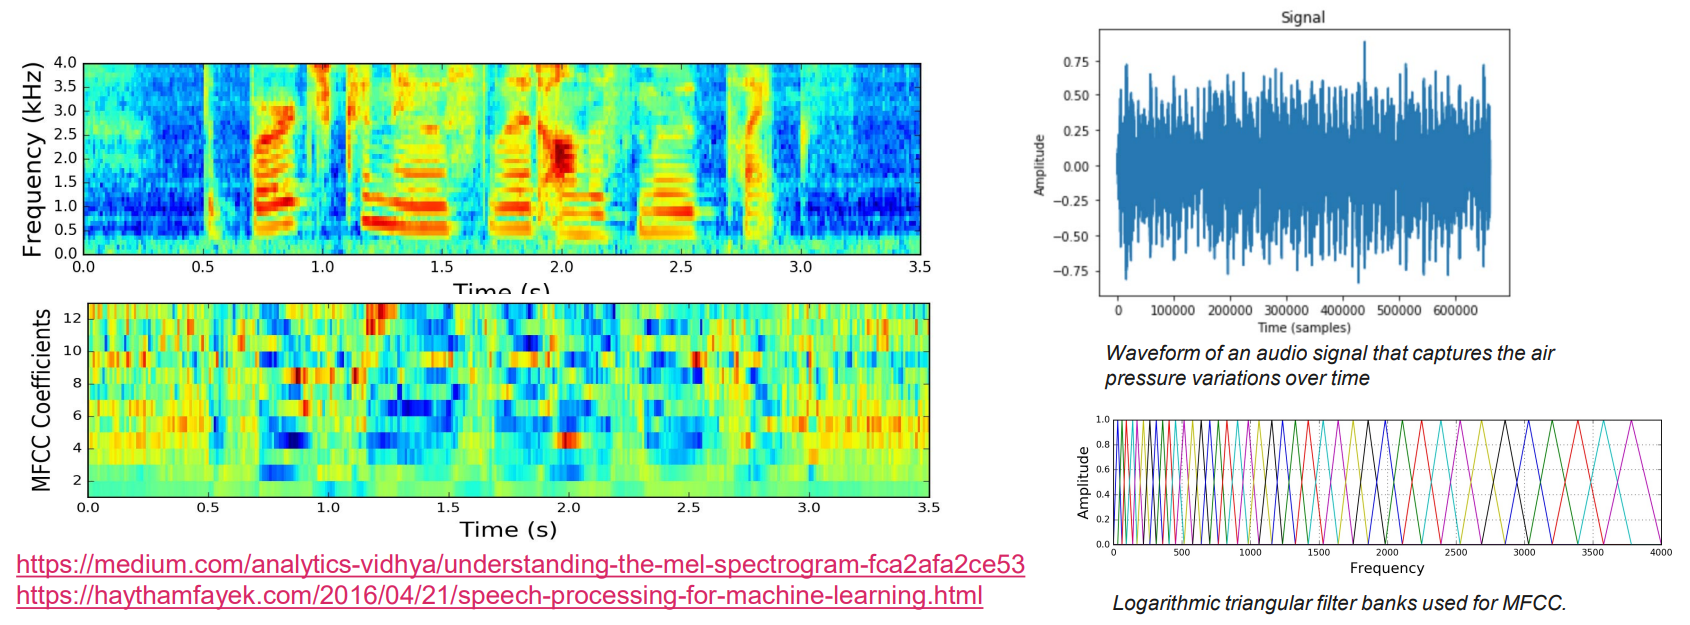
\includegraphics[width = \columnwidth]{figures/07/MFCC.png}
\end{figure}